%!TEX program = <lualatex>
\documentclass[12pt]{article}


\usepackage[utf8]{inputenc}
\usepackage[english]{babel}
\usepackage{csquotes}
\usepackage{graphicx}
\usepackage{indentfirst}
\usepackage{fontspec}
\usepackage{fancyhdr}
\usepackage{titling}
\usepackage{lipsum}

\usepackage[
backend=biber,
style=apa,
]{biblatex}

\usepackage[style=iso]{datetime2}

\usepackage{geometry}
\geometry{a4paper, margin=1in}

\addbibresource{INIT.bib}

\setlength{\parindent}{0.5in}
\renewcommand{\baselinestretch}{2}
\setlength{\headheight}{15pt}

\title{%
	INIT \\
	\large Individually Neurostimulated Inhibition Training for AUD}

\author{Andrea Häfliger, Olivier Ulrich, Konstantinos Zervas}

\pagestyle{fancy}
\fancyhead{}
\fancyhead[R]{INIT}
\fancyfoot{}
\fancyfoot[R]{\thepage}
\fancyfoot[L]{\theauthor}

\begin{document}

\pagestyle{fancy}
\thispagestyle{empty}

\maketitle
\newpage
\tableofcontents
\newpage

\section{Research Plan: Summary}

The proposed study will evaluate the potential of network-targeted brain stimulation to increase the efficacy of inhibition training protocols in treating alcohol use disorder. By comparing inhibition training accompanied by individually targeted transcranial magnetic stimulation with sham TMS, conventional rTMS, a standalone inhibition training protocol, and a control group receiving standard care in AUD treatment, we aim to assess both the feasibility of such a regimen, as well as its effect on treatment outcomes relating to AUD. The inhibition training uses a modified Go/NoGo task to improve patients' ability to inhibit pre-potent responses toward alcoholic stimuli and has been shown to reduce alcohol intake \parencite{houbenBeerNogoLearning2012}. Performance differences between AUD patients and healthy controls in regular Go/NoGo tasks using alcohol related stimuli have been shown to depend on neuronal circuitry commonly thought of being involved in inhibitory processes \parencite{czaplaAlcoholdependentPatientsShow2017,volkowAddictionScienceUncovering2014,simmondsMetaanalysisGoNogo2008,luijtenSystematicReviewERP2014}. Network-targeted TMS has been suggested to be able to modulate neuronal activity in deeper lying brain regions, overcoming a critical hurdle of non-invasive brain stimulation \parencite{momiCognitiveEnhancementNetworkTargeted2020}. By using critical regions in inhibitory processes to build a functional connectivity map of inhibition we can identify individual cortical regions in each participant that can serve as gateways for TMS to target the underlying inhibitory network and thus increase inhibitory performance. This allows us to evaluate whether this facilitated inhibitory control can improve the effects of inhibition training for AUD.

\section{Research Plan}


\subsection{State of research}
Alcohol Use Disorder (AUD) is a major public risk factor for premature mortality in industrialised western countries and is responsible for more than 200 medical conditions including chronic disease and injury. In 2016, the excessive use of alcohol was responsible for 3 million deaths worldwide. AUD ranks third on the list of common risk factors for morbidity, after cigarette smoking and hypertension, but there are few effective therapies to curb it, the usual treatment consisting of specialised relapse prevention programs. 

\textcite{houbenBeerNogoLearning2012} presented a modified Go/NoGo task that bears the potential of reducing alcohol consumption. Other trainings, such as the Cue Avoidance Training, in which patients consistently push alcoholic stimuli away from themselves with a joystick, didn’t show greater effects than a normal Go/No-Go task \parencite{dilemmaCueAvoidanceTraining2017}. In a recent study, three different tasks, a Beer-Go/No-Go a Stop Signal task and a combined task were compared to a control condition and a Brief Alcohol Intervention (BAI). In the Beer-Go/No-Go task the No-Go trials were always paired with a picture of a glass of beer, but the beer itself was not a cue for the appropriate reaction. With the Stop-Signal Task the participants had to withhold a response if the cue changed colour after its presentation. In the combined condition participants had to stop their response if the image changed to a beer stimulus. None of the conditions produced a greater reduction in alcohol consumption per week than the control condition \parencite{smithCurrentFormsInhibitory2017}. 

The first study to investigate the effects of an expanded alcohol inhibition training on a clinical population used six different training sessions within two weeks. Difficulties were varied along the Go/No Go ratio. Every participant had to undergo one of three different alcohol inhibition trainings: Either on of the two alcohol inhibition trainings (alc-IT) with a Go/NoGo ratio of (50/50) or (75/25) or a control training, where the alcoholic or neutral cue was not systematically paired with the Go or NoGo trials. The increase in abstinent days in the alc-IT group with a Go/NoGo ratio of (75/25) was more pronounced than in the control and the alc-IT (50/50) group, but the specific underlying mechanism and the mediating neurophysiological changes still remain unclear \parencite{tschuemperlinLearningResistUrge2019}, even though other studies have investigated the neuronal basis of inhibition.

An fMRI study that focused on the differences in the neural response during a Go/NoGo task between heavy and light drinkers found that heavy drinkers showed a significant higher BOLD signal during NoGo trials in the rDLPFC, ACC and insula than light drinkers. This finding was explained by the fact that heavy drinkers have to allocate more resources for response inhibition towards alcoholic stimuli. Regardless of the higher activation in these networks, heavy drinkers performed worse on the Go/NoGo task \parencite{amesNeuralCorrelatesGo2014}. A similar performance difference was found in a study of \textcite{noelAlcoholCuesIncrease2007}, where alcoholics made more commission and omission errors in an alcohol inhibition task \parencite{noelAlcoholCuesIncrease2007}. The anatomical and functional regions found in the study of \textcite{amesNeuralCorrelatesGo2014} partially coincide with Volkow's network of inhibitory control and executive functions consisting of the dlPFC, ACC, IFC and lateral OFC \parencite{volkowAddictionScienceUncovering2014}. Although newer studies suggest that the cerebellum is also likely involved in inhibitory control, especially in proactive and reactive control \parencite{clarkCerebellarContributionsProactive2020}. These findings point to a network of critical regions involved in inhibitory control that seems to be more active in people with AUD, even though it is not entirely clear how its activity influences inhibitory performance.

A promising tool to enhance cognitive functions in neuroscience is transcranial magnetic stimulation (TMS). In its beginnings, TMS was intended to be used as a method to apply virtual lesions. It was used to investigate the effects of the interruption of distinct brain regions on task performance. Nowadays, TMS is widely used in clinical and experimental settings to enhance cognitive performance \parencite{luberEnhancementHumanCognitive2014}. Most online protocols use inhibitory repetitive TMS (rTMS) protocols following the virtual lesion approach. Offline protocols can be either excitatory or inhibitory, depending on the pulse frequency; frequencies under 1 Hz are usually inhibitory and those above 1 Hz are excitatory \parencite{beynelEffectsOnlineRepetitive2019}. Various studies were able to evoke a reduction in alcohol cravings by applying a high frequency (10 Hz) rTMS stimulation to the rDLPFC \parencite{antonelliTranscranialMagneticStimulation2021}. Still, the neural mechanisms mediating the effects of rTMS on cravings and reductions in alcohol consumption are not yet completely understood. 

Since TMS can only penetrate a small distance into brain tissue, subcortical regions seem to be unaffected by TMS stimulation. A promising new approach in applying TMS pulses to subcortical regions and to alter cortico-subcortical connectivity is the calculation of cortical stimulation locations on the basis of resting state fMRI connectivity analyses \parencite{wangTargetedEnhancementCorticalhippocampal2014}. By applying this technique, the research group around Joel Voss found a way to enhance cortico-hippocampal network connectivity and in turn improve memory encoding. To extract a suitable cortical stimulation site, they calculated resting state fMRI connectivity analyses, then defined a target or seed region, in this case the hippocampus, and searched for cortical voxels that were maximally functionally connected to these target regions \parencite{hermillerEvidenceImmediateEnhancement2020}. Following the same principle, \textcite{howardTargetedStimulationHuman2020} used connectivity analyses to define a stimulation site over the DLPFC that was highly connected with the OFC \parencite{howardTargetedStimulationHuman2020}. 

To our knowledge, no studies have yet employed TMS in combination with an inhibition training to alter therapeutic outcomes. Neither has the potential of altering cortico-striatal connectivity with resting state fMRI connectivity targeted cortical regions and rTMS been tested.

\subsection{Detailed research plan}


\subsubsection{Objectives and hypotheses}

This project's objectives are essentially twofold: for one, we intend to further the understanding of the neuronal circuitry involved in inhibitory processes related to alcohol specific stimuli by investigating functional connections between various subcortical regions known to be implicated in the act of inhibitory control, as well as search for further connections linking these areas to cortical regions that may be used as targets for non-invasive brain stimulation. Secondly, we intend to use these findings to identify patient specific cortical gateway regions to stimulate during established inhibition training session in order to investigate the stimulation's potential to bolster the improvement in inhibitory control performance evoked by these trainings.

The functional and connectional insights attained through the pre- and post-measures bear the potential of both broadening the spectrum of potentially relevant inhibitory circuitry, and deepening our understanding of the specific involvements and interactions between already identified areas in inhibition processes. Exemplarised through the interaction model of addiction and inhibition proposed by \textcite{volkowAddictionScienceUncovering2014}, this may result in a proposed inclusion of further regions, hitherto not having been directly implicated in these processes, or additional connections between already included regions. Due to the intervention based approach and the thorough nature of the proposed neurophysiological measurements in this study, a quantification of functional connections and their implications in inhibitory performance specifically and in addiction more generally is a possibility as well.

The aforementioned intervention based approach forms the framework to realise the second of the proposed project's goals; evaluating the potential of transcranial magnetic stimulation in increasing the effects of inhibition training in patients suffering from AUD. Existing research in this field has investigated both the effect of non-invasive brain stimulation on addiction in general \parencite{antonelliTranscranialMagneticStimulation2021,mostafaviNoninvasiveBrainStimulation2020,zhangEffectsRepetitiveTranscranial2019}, and its use in identifying and describing neuronal circuitry involved in inhibition \parencite{naim-feilCorticalInhibitionMotor2016,quoilinNeuralBasesInhibitory2021}. To date, however, there has not been any systematic inquiry into the effectiveness of TMS or other non-invasive brain stimulation in conjunction with behavioural inhibition training paradigms. Our study has set its sight on this specific niche and aims to go one step further by also including network targeting methods to determine optimal TMS application and its effect on inhibition training. These methods have been shown to allow targeting of specific networks usually unreachable by TMS by utilising the functional connectivity underlying the circuitry in question and has been shown to be a fruitful method to improve cognitive performance in tasks related to the targeted networks \parencite{momiCognitiveEnhancementNetworkTargeted2020}. Based on the framework of \textcite{volkowAddictionScienceUncovering2014}, we thus posit that such network targeted TMS may be well suitable to target the neural circuitry involved in inhibition and thus has the potential of being an effective addition to the current, purely behavioural tasks used in inhibition training programs.

\subsubsection{Participants}

Meta analyses failed to show significant effect sizes in studies that used TMS to treat patients with AUD \parencite{mostafaviNoninvasiveBrainStimulation2020, zhangEffectsRepetitiveTranscranial2019}. Since the planned intervention is fairly extensive, we aspire to produce results proportional to the expected effort. To calculate the required sample size using G*Power, we thus chose a small to medium effect size of f=0.2, which, along with a minimum power of 0.8 and the default setting for the expected correlation among the repeated measures of 0.5, resulted in a suggested sample size of 230 total, or 46 participants per condition. \parencite{faulStatisticalPowerAnalyses2009, bhaleraoSampleSizeCalculation2010}. 
To avoid any interferences from differences in lateralisations of language, only right-handed patients will be recruited. Exclusion criteria are defined as follows:

\begin{itemize}
\item No tattoos in the head area 
\item No MR-compliant iron/metals in/on the body
\item No dental implants (retainers are allowed)
\item No neurological or psychiatric history or current medical conditions, e.g. epilepsy
\item No Intake of any medication that is likely to lower seizure threshold
\item No excessive drug use besides alcohol
\item No diabetes, heart diseases or current infections
\item No sleep, memory or concentration disorders or sleep deprivation
\item No claustrophobia or sensitivity to noise
\item No dizziness or migraine 
\item No near-sightedness or far-sightedness if not corrected by currently valid (recently prescribed) contact lenses
\item No participation in previous studies with the same content  
\item No vaccinations in the near future 
\end{itemize}

All participants will be recruited among newly admitted patients diagnosed with AUD in two substance-abuse clinics near Bern: Klinik Südhang and Klinik Selhofen. Upon first checking into the clinic, patients receive an information booklet explaining the aims of the study and sign a declaration of consent about the collection and use of data required in this project. They are also asked to fill out a questionnaire about the in- and exclusion criteria and about their agreement to be informed about incidental findings. Failure to do so will exclude them from participating.

All participants willing to take part in the study will be informed of the complete procedures that will take place including the MRI, rTMS, Go/No-Go task and the follow up questionnaire including the HDL and the TLFB.

\subsubsection{Study design, procedures, and measures}

To allow for a thorough later analysis of the trainings' effects, we will initially conduct a baseline measure of both inhibitory control as well as the individuals' reactions to alcoholic stimuli during an fMRI scan. Inhibitory control is measured by a modified Go/NoGo task using alcohol related stimuli contrasted with images of non-alcoholic beverages. These kinds of Go/NoGo task find widespread use in the assessment of inhibitory control in a context of AUD and provide a robust measure to assess an individual's ability to inhibit an automated response to alcohol related information \parencite{amesNeuralCorrelatesGo2014,bowleyEffectsInhibitoryControl2013,roseEffectsAlcoholInhibitory2008,simmondsMetaanalysisGoNogo2008}. Like the Go/NoGo task used in the actual inhibition training \parencite{houbenBeerNogoLearning2012}, this task uses letters presented alongside the stimuli as Go/NoGo signals, with both types of stimuli appearing in tandem with both Go and NoGo cues. The participants are thus instructed to press a button whenever a Go signal appears, but not when a NoGo signal does. The stimuli are presented in a randomised order and a four to one ratio of Go and NoGo signals, respectively. This ratio has been shown to ensure the formation of a pre-potent response tendency towards Go signals \parencite{amesNeuralCorrelatesGo2014}. Since the task will be performed during an fMRI scan, the timings of both the trials and the inter trial duration will be jittered.

Each participant's neurophysiological reaction to alcoholic stimuli will be measured using a simple cue reactivity task consisting of alcoholic stimuli. 

These baseline measures will be conducted during an fMRI scan, following a T1 weighted structural scan to gather anatomical information on each participant. Based on the fMRI data collected during both the cue reactivity task and the Go/NoGo task, BOLD signals will be analysed to assess individual neurophysiological activity. For the Go/NoGo task, BOLD activity during successfully inhibited responses (correctly rejected NoGo trials) and correctly answered Go trials, as well as the interaction between all alcoholic NoGo trials contrasted with all alcoholic Go trials and all neutral NoGo trials contrasted with all neutral Go trials. Contrasts in the cue reactivity task will be formed between the fixation trials and the alcohol stimulus trials, thus providing information on the location and extent of the individual physiological response.

The functional data obtained during the Go/NoGo task will be used to conduct connectivity analyses between inhibitory regions and a series of candidate regions closer to the surface of the brain. These analyses are intended to identify potential gateway regions, which can be used as targets of non-invasive brain stimulation and would propagate the stimulation's effects to the lower laying inhibitory regions that cannot be targeted directly. The aim is to find the most positively correlated nodes of a functional connectivity map calculated from individual seed regions. The seeds will be chosen based on the BOLD activity during the inhibitory control task.

After applying the interventions, we will assess the behavioural effects of the different programs by again measuring inhibitory control with a Go/NoGo-Task. Performances of the pre- and post-measures will be compared to evaluate the success of the interventions conducted. This will form our main outcome measure as it directly addresses the immediate effects of the different types of inhibition trainings being tested.
The second outcome measure regards cue reactivity, whose relevant post-intervention data will again be collected during an fMRI scan, with differences between the two measurements being the outcomes of interest.
As a third key feature, we examine changes of cortical thickness over the time of intervention. This will be allow us to explore whether the training of inhibitory control can affect structural characteristics.
To assess whether these intervention have long term-impacts, the participants are asked to fill out two questionnaires 6 months after leaving the substance abuse clinics: The Health and Daily Living Form \parencite{moosHealthDailyLiving1986} is an overall assessment of factors that influence health, such as substance consumption and depression; the Alcohol Timeline Followback \parencite{sobellAlcoholTimelineFollowback1995} requires participants to retrospectively recall their daily drinking to get an estimate of the extent of alcohol consumption.

\subsubsection{Data analysis}

Based on our hypotheses, we expect to find effects both within the experimental groups, due to the general effectiveness of AUD interventions, and between them, due to the potential of increasing training effectiveness through TMS. To test for these effects, we can construct multiple ANOVAs based on our outcome measures using time as a within factor and the experimental groups as a between factor. This allows us to investigate any significant interactions between time and group for each measure in detail, using post-hoc group comparisons to asses the iterative effectiveness of each of the proposed interventions.

For each of the outcome measures, different within factors need to be added, for the Go/NoGo task and the cue reactivity tasks the within factors will include the stimulus type and time, and for the structural data it will only include time.

\subsubsection{Ethical considerations}
All inclusion and exclusion criteria that ensure the participants are fit to enrol in the study are listed above.

As there is a shamTMS condition in our study design to exclude any placebo effects stemming from the mere fact that something is done with the participants, those receiving shamTMS will be informed in the same manner as those in the experimental condition. This is the only sort of deception included in this study. 

The MRI sessions do not pose any health risks, however, the narrowness of the scanner tube and its noise during application of RF pulses harbours the risk of rendering participants uncomfortable. To address the noise, participants will wear earplugs. While entering the MRI tube, some participants may experience dizziness as their vestibular organs adapt to the stronger magnetic field. In the improbable case that they feel unwell during the scans, an emergency switch is present that can be used at any time to stop the scanning process. All the MR scans will be supervised by experienced medical technicians. 

Participants receive information about the procedure for incidental findings: if potential neurological abnormalities are detected, they are informed and given instructions about suggested necessary steps to be taken, e.g. a neurological examination.

The TMS sessions will be supervised by a medical doctor but do not in itself harbour any major health risk. The application of the electric current through the coil and thus the extension of the magnetic fields into the skull can sometimes cause an itching pain on the cranial skin, and in some cases participants report nausea or involuntary movements across the face. In rare instances, TMS can induce syncope, which does not constitute a life-threatening condition. To mitigate the risk of epileptic seizures, participants with elevated seizure risk due to seizure threshold lowering medication or family history of epileptic seizures will be excluded from the study. After each session, participants are offered the chance to consult a medical doctor in case they feel unwell after stimulation. 

Should the confrontation with alcoholic stimuli induce strong cravings, participants may seek support from psychologists at their respective substance abuse clinics.

\subsection{Timetable and milestones}
A rough timeline of the research project is shown below. Short-term adjustments are possible at any time.

\begin{figure}[h]
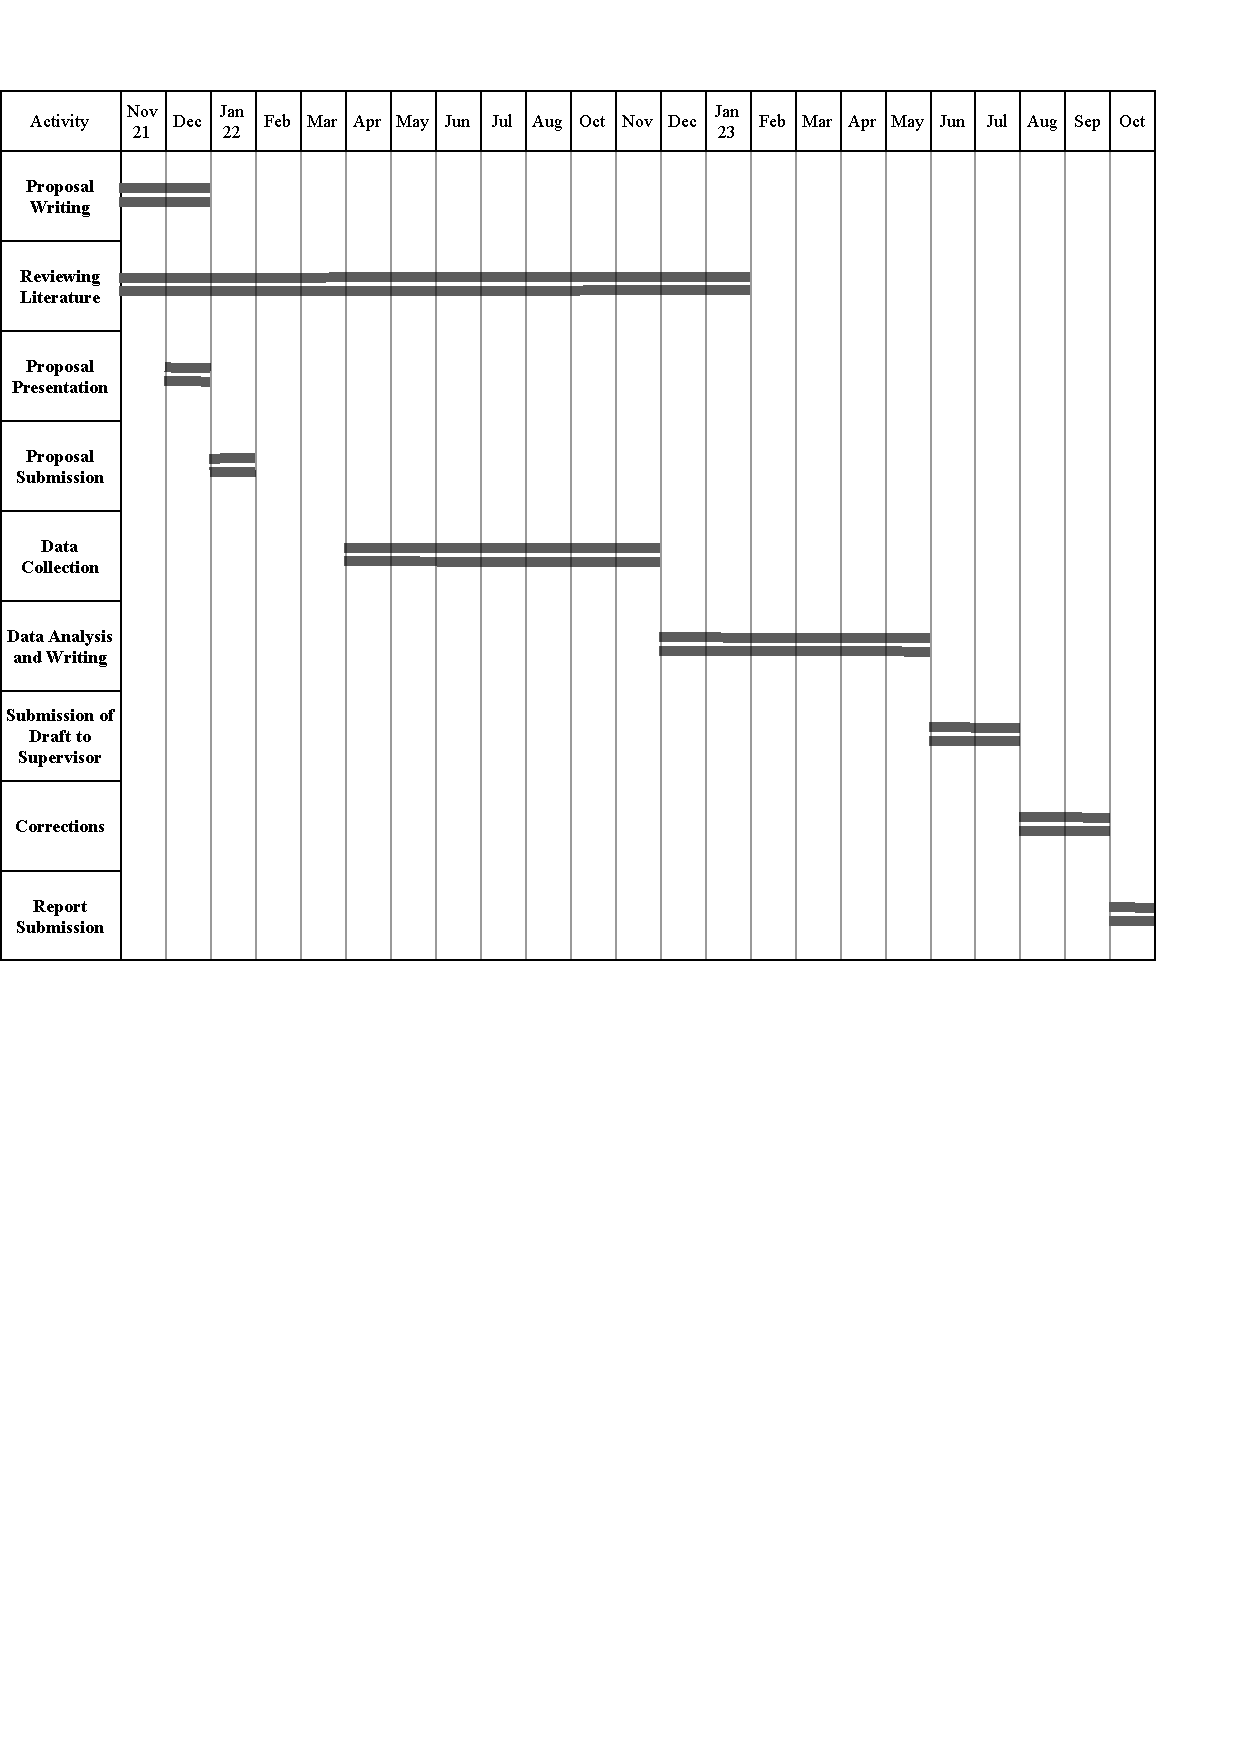
\includegraphics[width=\textwidth,keepaspectratio]{Timetable2.pdf}
\caption{Timetable of the proposed research plan.}
\end{figure}

\subsection{Significance of planned research to the scientific community and to potential users}
In Switzerland, 250’000 to 300’000 individuals suffer from AUD. Yearly, abusive alcohol consumption causes public costs of 2.8 billion Swiss francs \parencite{AlkoholUndAlkoholpravention2021}. There are numerous institutions and therapy programs, however only 40\% of patients are still abstinent one year after stationary treatment \parencite{moggiSubstanceUseDisorder2007}. These facts suggest that improving established treatment programs should be a top priority in substance abuse research. The proposed study examines different trainings that add to the standard care in AUD treatment and could offer an individualised solution for patients whose conditions fail to improve through standardised programs. 
Furthermore, this study can provide further insights on the role of inhibitory control in abstinence. Previous findings (e.g. about inhibitory networks) can be replicated and underlying mechanisms explored.
Individualised rTMS could also be of use in numerous fields of research distinct from addiction treatment, and this study may serve as an example of this promising method and give legitimation to the exploration of its effects in other fields.
Conclusively, this project would be of major significance for both public health, and neuropsychological research.

\printbibliography  
\end{document}